\documentclass[12pt]{article}

\usepackage{amsmath}
\usepackage{amssymb}
\usepackage{physics}
\usepackage{enumitem}
\usepackage{tikz}
\usetikzlibrary{arrows.meta,angles,quotes,calc}
\usepackage{geometry}
\geometry{margin=1in}

\begin{document}

\begin{flushleft}
{\Large \textbf{SET 20 — Final Fully Corrected Version}}
\end{flushleft}

\vspace{0.5cm}

%%%%%%%%%%%%%%%%%%%%%%%%%%%%%%%%%%%%%%%%%%%%%%%%%%%%%%%%%%%%
\textbf{Q1.}

A wedge of mass $M$ is placed on a smooth horizontal surface. 
An incline of angle $\theta$ is fixed on the wedge. 
A small block of mass $m$ is placed on the incline and is connected 
by a light inextensible string passing over a smooth pulley fixed rigidly 
at the top of the wedge to another block of mass $m$ hanging vertically. 

All surfaces are frictionless. The pulley is fixed to the wedge and moves along with it. 
The system is released from rest. 
Find the acceleration of the wedge.

\begin{center}
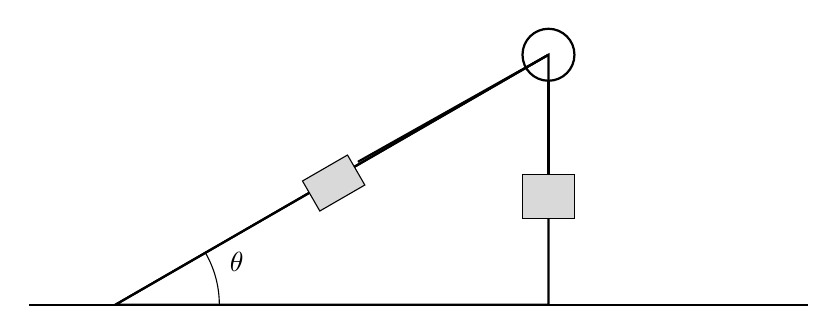
\begin{tikzpicture}[scale=1.1]

% Ground
\draw[thick] (-1,0) -- (8,0);

% Incline angle chosen exactly 30 degrees
\def\angle{30}
\def\base{5}
\def\height{2.886} % 5*tan(30°)

% Wedge
\draw[thick] (0,0) -- (\base,0) -- (\base,\height) -- cycle;

% Incline
\draw[thick] (0,0) -- (\base,\height);

% Angle theta
\draw (1.2,0) arc (0:\angle:1.2);
\node at (1.4,0.5) {$\theta$};

% Block on incline (rotated correctly)
\begin{scope}[rotate around={\angle:(2.5,1.44)}]
\draw[fill=gray!30] (2.2,1.2) rectangle (2.8,1.6);
\end{scope}

% Pulley
\draw[thick] (\base,\height) circle (0.3);

% String along incline
\draw[thick] (2.8,1.65) -- (\base,\height);

% Vertical string
\draw[thick] (\base,\height-0.3) -- (\base,1.5);

% Hanging block
\draw[fill=gray!30] (\base-0.3,1.0) rectangle (\base+0.3,1.5);

\end{tikzpicture}
\end{center}

Options:

(A) $\displaystyle \frac{2mg\sin\theta}{M+2m-m\cos^2\theta}$

(B) $\displaystyle \frac{2mg\sin\theta}{M+2m}$

(C) $\displaystyle \frac{mg\sin\theta}{M+m}$

(D) $\displaystyle \frac{2mg\sin\theta}{M+2m+m\cos^2\theta}$

\vspace{0.7cm}

%%%%%%%%%%%%%%%%%%%%%%%%%%%%%%%%%%%%%%%%%%%%%%%%%%%%%%%%%%%%
\textbf{Q2.}

A particle of mass $m$ moves under a central force 
\[
F(r) = -\frac{k}{r^2} + \frac{\alpha}{r^3},
\]
where $k$ and $\alpha$ are positive constants. 
Determine the radius of the stable circular orbit.

Options:

(A) $\displaystyle \frac{\alpha}{k}$

(B) $\displaystyle \frac{k}{\alpha}$

(C) $\displaystyle \sqrt{\frac{\alpha}{k}}$

(D) $\displaystyle \frac{\alpha}{2k}$

\vspace{0.7cm}

%%%%%%%%%%%%%%%%%%%%%%%%%%%%%%%%%%%%%%%%%%%%%%%%%%%%%%%%%%%%
\textbf{Q3.}

A uniform solid cylinder of mass $M$ and radius $R$ is placed on a rough horizontal plank. 
The plank is accelerated horizontally with constant acceleration $a$. 
The coefficient of friction is sufficient to ensure pure rolling without slipping. 
Find the acceleration of the centre of mass of the cylinder relative to the ground.

Options:

(A) $\frac{2a}{3}$

(B) $\frac{a}{2}$

(C) $a$

(D) $\frac{3a}{2}$

\vspace{0.7cm}

%%%%%%%%%%%%%%%%%%%%%%%%%%%%%%%%%%%%%%%%%%%%%%%%%%%%%%%%%%%%
\textbf{Q4.}

A parallel plate capacitor of capacitance $C$ is connected to a battery 
maintaining constant potential $V$. 
A dielectric slab of dielectric constant $K$ completely fills the space 
between the plates and is then slowly removed. 
Find the work done by the battery during this process.

Options:

(A) $\frac{1}{2}CV^2(K-1)$

(B) $\frac{1}{2}CV^2\left(1-\frac{1}{K}\right)$

(C) $CV^2(K-1)$

(D) $\frac{1}{2}CV^2\left(\frac{1}{K}-1\right)$

\vspace{0.7cm}

%%%%%%%%%%%%%%%%%%%%%%%%%%%%%%%%%%%%%%%%%%%%%%%%%%%%%%%%%%%%
\textbf{Q5.}

Two isolated conducting spheres of radii $R$ and $4R$ are placed far apart. 
They are connected by a thin conducting wire and a total charge $Q$ is supplied. 
Find the charge on the larger sphere after electrostatic equilibrium is established.

Options:

(A) $\frac{4Q}{5}$

(B) $\frac{Q}{2}$

(C) $\frac{Q}{4}$

(D) $\frac{Q}{5}$

\vspace{0.7cm}

%%%%%%%%%%%%%%%%%%%%%%%%%%%%%%%%%%%%%%%%%%%%%%%%%%%%%%%%%%%%
\textbf{Q6.}

A uniformly charged rod of length $2L$ lies along the x-axis. 
Find the electric field at a point located at a distance $a$ from its centre 
on the perpendicular bisector, assuming $a \ll L$.

Options:

(A) Proportional to $\frac{1}{a}$

(B) Proportional to $\frac{1}{a^2}$

(C) Approximately constant

(D) Zero

\vspace{0.7cm}

%%%%%%%%%%%%%%%%%%%%%%%%%%%%%%%%%%%%%%%%%%%%%%%%%%%%%%%%%%%%
\textbf{Q7.}

A conducting rod of length $l$ slides without friction on two parallel conducting rails 
placed in a uniform magnetic field $B$ perpendicular to the plane. 
The circuit has total resistance $R$ and inductance $L$. 
Determine the time dependence of the current in the circuit.

Options:

(A) Exponential rise

(B) Linear rise

(C) Constant

(D) Oscillatory

\vspace{0.7cm}

%%%%%%%%%%%%%%%%%%%%%%%%%%%%%%%%%%%%%%%%%%%%%%%%%%%%%%%%%%%%
\textbf{Q8.}

A charged particle moves in a uniform magnetic field in circular motion. 
It suddenly receives a radial impulse. 
Describe its subsequent motion.

Options:

(A) Circular motion with a new radius

(B) Spiral inward

(C) Spiral outward

(D) Linear motion

\vspace{0.7cm}

%%%%%%%%%%%%%%%%%%%%%%%%%%%%%%%%%%%%%%%%%%%%%%%%%%%%%%%%%%%%
\textbf{Q9.}

A light ray is incident at a small angle $\theta$ on a slab of refractive index $\mu$ 
and thickness $t$. 
Find the lateral shift produced for small $\theta$.

Options:

(A) $t\theta\left(1-\frac{1}{\mu}\right)$

(B) $t\theta(1-\mu)$

(C) $\mu t\theta$

(D) $\frac{t\theta}{\mu}$

\vspace{0.7cm}

%%%%%%%%%%%%%%%%%%%%%%%%%%%%%%%%%%%%%%%%%%%%%%%%%%%%%%%%%%%%
\textbf{Q10.}

A thin convex lens and a plane mirror are placed coaxially. 
Light from an object placed on the principal axis passes through the lens, 
reflects from the mirror and again passes through the lens. 
Find the condition for the final image to coincide with the object.

Options:

(A) $f = R$

(B) Net optical power zero

(C) $f = \frac{R}{2}$

(D) $f = 2R$

\vspace{0.7cm}

%%%%%%%%%%%%%%%%%%%%%%%%%%%%%%%%%%%%%%%%%%%%%%%%%%%%%%%%%%%%
\textbf{Q11.}

In a double slit experiment with slit width $a$ and separation $d$, 
determine the condition for a missing interference maximum.

Options:

(A) $\frac{d}{a} = \frac{1}{2}$

(B) $a = d$

(C) $\frac{d}{a} = n$

(D) $d = \frac{a}{n}$

\vspace{0.7cm}

%%%%%%%%%%%%%%%%%%%%%%%%%%%%%%%%%%%%%%%%%%%%%%%%%%%%%%%%%%%%
\textbf{Q12.}

In a photoelectric experiment, the graph of stopping potential versus frequency 
is a straight line of slope $S$. 
Determine Planck's constant in terms of $S$.

Options:

(A) $h = \frac{S}{e}$

(B) $h = eS$

(C) $h = \frac{e}{S}$

(D) $h = S$

\vspace{0.7cm}

%%%%%%%%%%%%%%%%%%%%%%%%%%%%%%%%%%%%%%%%%%%%%%%%%%%%%%%%%%%%
\textbf{Q13.}

In the Bohr model of hydrogen atom, determine the angular momentum 
of the electron in the fifth orbit.

Options:

(A) $5\hbar$

(B) $\frac{5}{2}\hbar$

(C) $10\hbar$

(D) $\hbar$

\vspace{0.7cm}

%%%%%%%%%%%%%%%%%%%%%%%%%%%%%%%%%%%%%%%%%%%%%%%%%%%%%%%%%%%%
\textbf{Q14.}

Two radioactive species with decay constants $\lambda_1$ and $\lambda_2$ 
are produced simultaneously. 
Determine the time at which their activities become equal.

Options:

(A) $\frac{1}{\lambda_1-\lambda_2}\ln\left(\frac{\lambda_1}{\lambda_2}\right)$

(B) $\frac{1}{\lambda_1+\lambda_2}$

(C) $\ln\left(\frac{\lambda_1}{\lambda_2}\right)$

(D) $\frac{1}{\lambda_1}$

\vspace{0.7cm}

%%%%%%%%%%%%%%%%%%%%%%%%%%%%%%%%%%%%%%%%%%%%%%%%%%%%%%%%%%%%
\textbf{Q15.}

A diode obeys the relation 
\[
I = I_0\left(e^{\frac{V}{\eta V_T}} -1\right).
\]
When a series resistance $R$ is present and $V \gg V_T$, 
determine the approximate current in the circuit.

Options:

(A) $\frac{V}{R}$

(B) $\frac{V-\eta V_T \ln\left(\frac{V}{I_0R}\right)}{R}$

(C) $\frac{V-\eta V_T}{R}$

(D) $I_0 e^{V/V_T}$

%%%%%%%%%%%%%%%%%%%%%%%%%%%%%%%%%%%%%%%%%%%%%%%%%%%%%%%%%%%%

\end{document}
